\documentclass{article}
\usepackage{graphicx} % Required for inserting images
\usepackage{amsmath}
\usepackage{amssymb}
\usepackage{float}
\usepackage{textgreek}
\usepackage{fancyhdr}
\usepackage{hyperref}

% vnořené popisky obrázků
\usepackage{subcaption}

% automatická konverze EPS 
\usepackage{graphicx} 
\usepackage{listings}
\usepackage{epstopdf}
\usepackage{xcolor}

\pagestyle{fancy}



\definecolor{codegreen}{rgb}{0,0.6,0}
\definecolor{codegray}{rgb}{0.5,0.5,0.5}
\definecolor{codepurple}{rgb}{0.58,0,0.82}
\definecolor{backcolour}{rgb}{0.95,0.95,0.92}

\lstdefinestyle{mystyle}{
    backgroundcolor=\color{backcolour},   
    commentstyle=\color{codegreen},
    keywordstyle=\color{magenta},
    numberstyle=\tiny\color{codegray},
    stringstyle=\color{codepurple},
    basicstyle=\ttfamily\footnotesize,
    breakatwhitespace=false,         
    breaklines=true,                 
    captionpos=b,                    
    keepspaces=true,                 
    numbers=left,                    
    numbersep=5pt,                  
    showspaces=false,                
    showstringspaces=false,
    showtabs=false,                  
    tabsize=2
}

\lstset{style=mystyle}






\title{ARI-HW\_10}
\author{Matěj Pinkas}
\date{27. April 2024}

\lhead{Pinkas Matěj}
\chead{ARI-HW\_10}
\rhead{27. April 2024}


\begin{document}

\maketitle

\section{Úkol}

\begin{itemize}
    \item[-] Zvolím si konstanty $a$ a $b$ z mého datumu narození: 10.01.2003
    \begin{align*}
        a &= 1 & b &= 1
    \end{align*}

    \item[-] Dopočítám konstantu $c$ ze zadání: 
    \begin{align*}
        c &= 4\left( \frac{a+b-2}{16}+1 \right) = 4
    \end{align*}

    \item[-] Ze zadání a vlastních čísel získám spojitý přenos: 
    \begin{align*}
        G_s(s) &= \frac{s+\frac{3}{2}c}{(s+c)(s-1)} = \frac{s+6}{(s+4)(s-1)}
    \end{align*}
    
    \item[-] Diskretizuji přenos $G_s(s)$ pomocí funkce $c2d(G_s,T_s)$ pro vzorkovací frekvenci $T_s = 0,05$ s:
    \begin{align*}
        G_d(z) = \frac{0,05365z-0,03971}{z^2-1,87z+0,8607} 
    \end{align*}
    
    \item[-] Zvolím si regulátor PI s přenosem:
    \begin{align*}
        PI(s) &= K_P + \frac{1}{s}K_I\\
        PS(z) &= K_P + \frac{1}{z-1}K_S
    \end{align*}

    \newpage
    \item[-] Pomocí funkce $rltool()$ provedu PID tunning přenosu:
    \begin{figure}[H]
        \centering
        \includegraphics[clip, width=0.70\textwidth]{rltool.png}
        \caption{RLTOOL a PID tunning}
        \label{fig:rltool}
    \end{figure}
    \item[] při řešení se snažím splnit překmit maximálně 30\% a dobu ustálení do 3 s 

    \item[-] Z tunningu získám konstanty:
    \begin{align*}
        K_P &= 9\\
        K_S &= 2
    \end{align*}

    \item[-] V kódu přidám regulátor a implementeaci anti-windupu:

    \begin{lstlisting}[language=Octave, caption=Část implementace]
    e = zeros(numel(t), 1);
    ssum = zeros(numel(t), 1);
    
    kp = 9;
    ks = 2;
    
    for k = 1:numel(t)
        y(k) = C*x_sys(k,:)'; % output of the system
    
        % == Your code goes here ==
        e(k) = r(k) - y(k); % PS controller input
        ssum(k + 1) = ssum(k) + e(k); 
        
        u(k) = kp*e(k) + ks*ssum(k+1); 
       
        if abs(u(k)) >= u_sat % anti-windup 
           u(k) = kp*e(k);
           ssum(k+1) = 0;
        end
       
        % Saturation of the input
        u(k) = max(min(u(k), u_sat), -u_sat);\end{lstlisting}
    


    

    \begin{figure}[H]
        \centering
        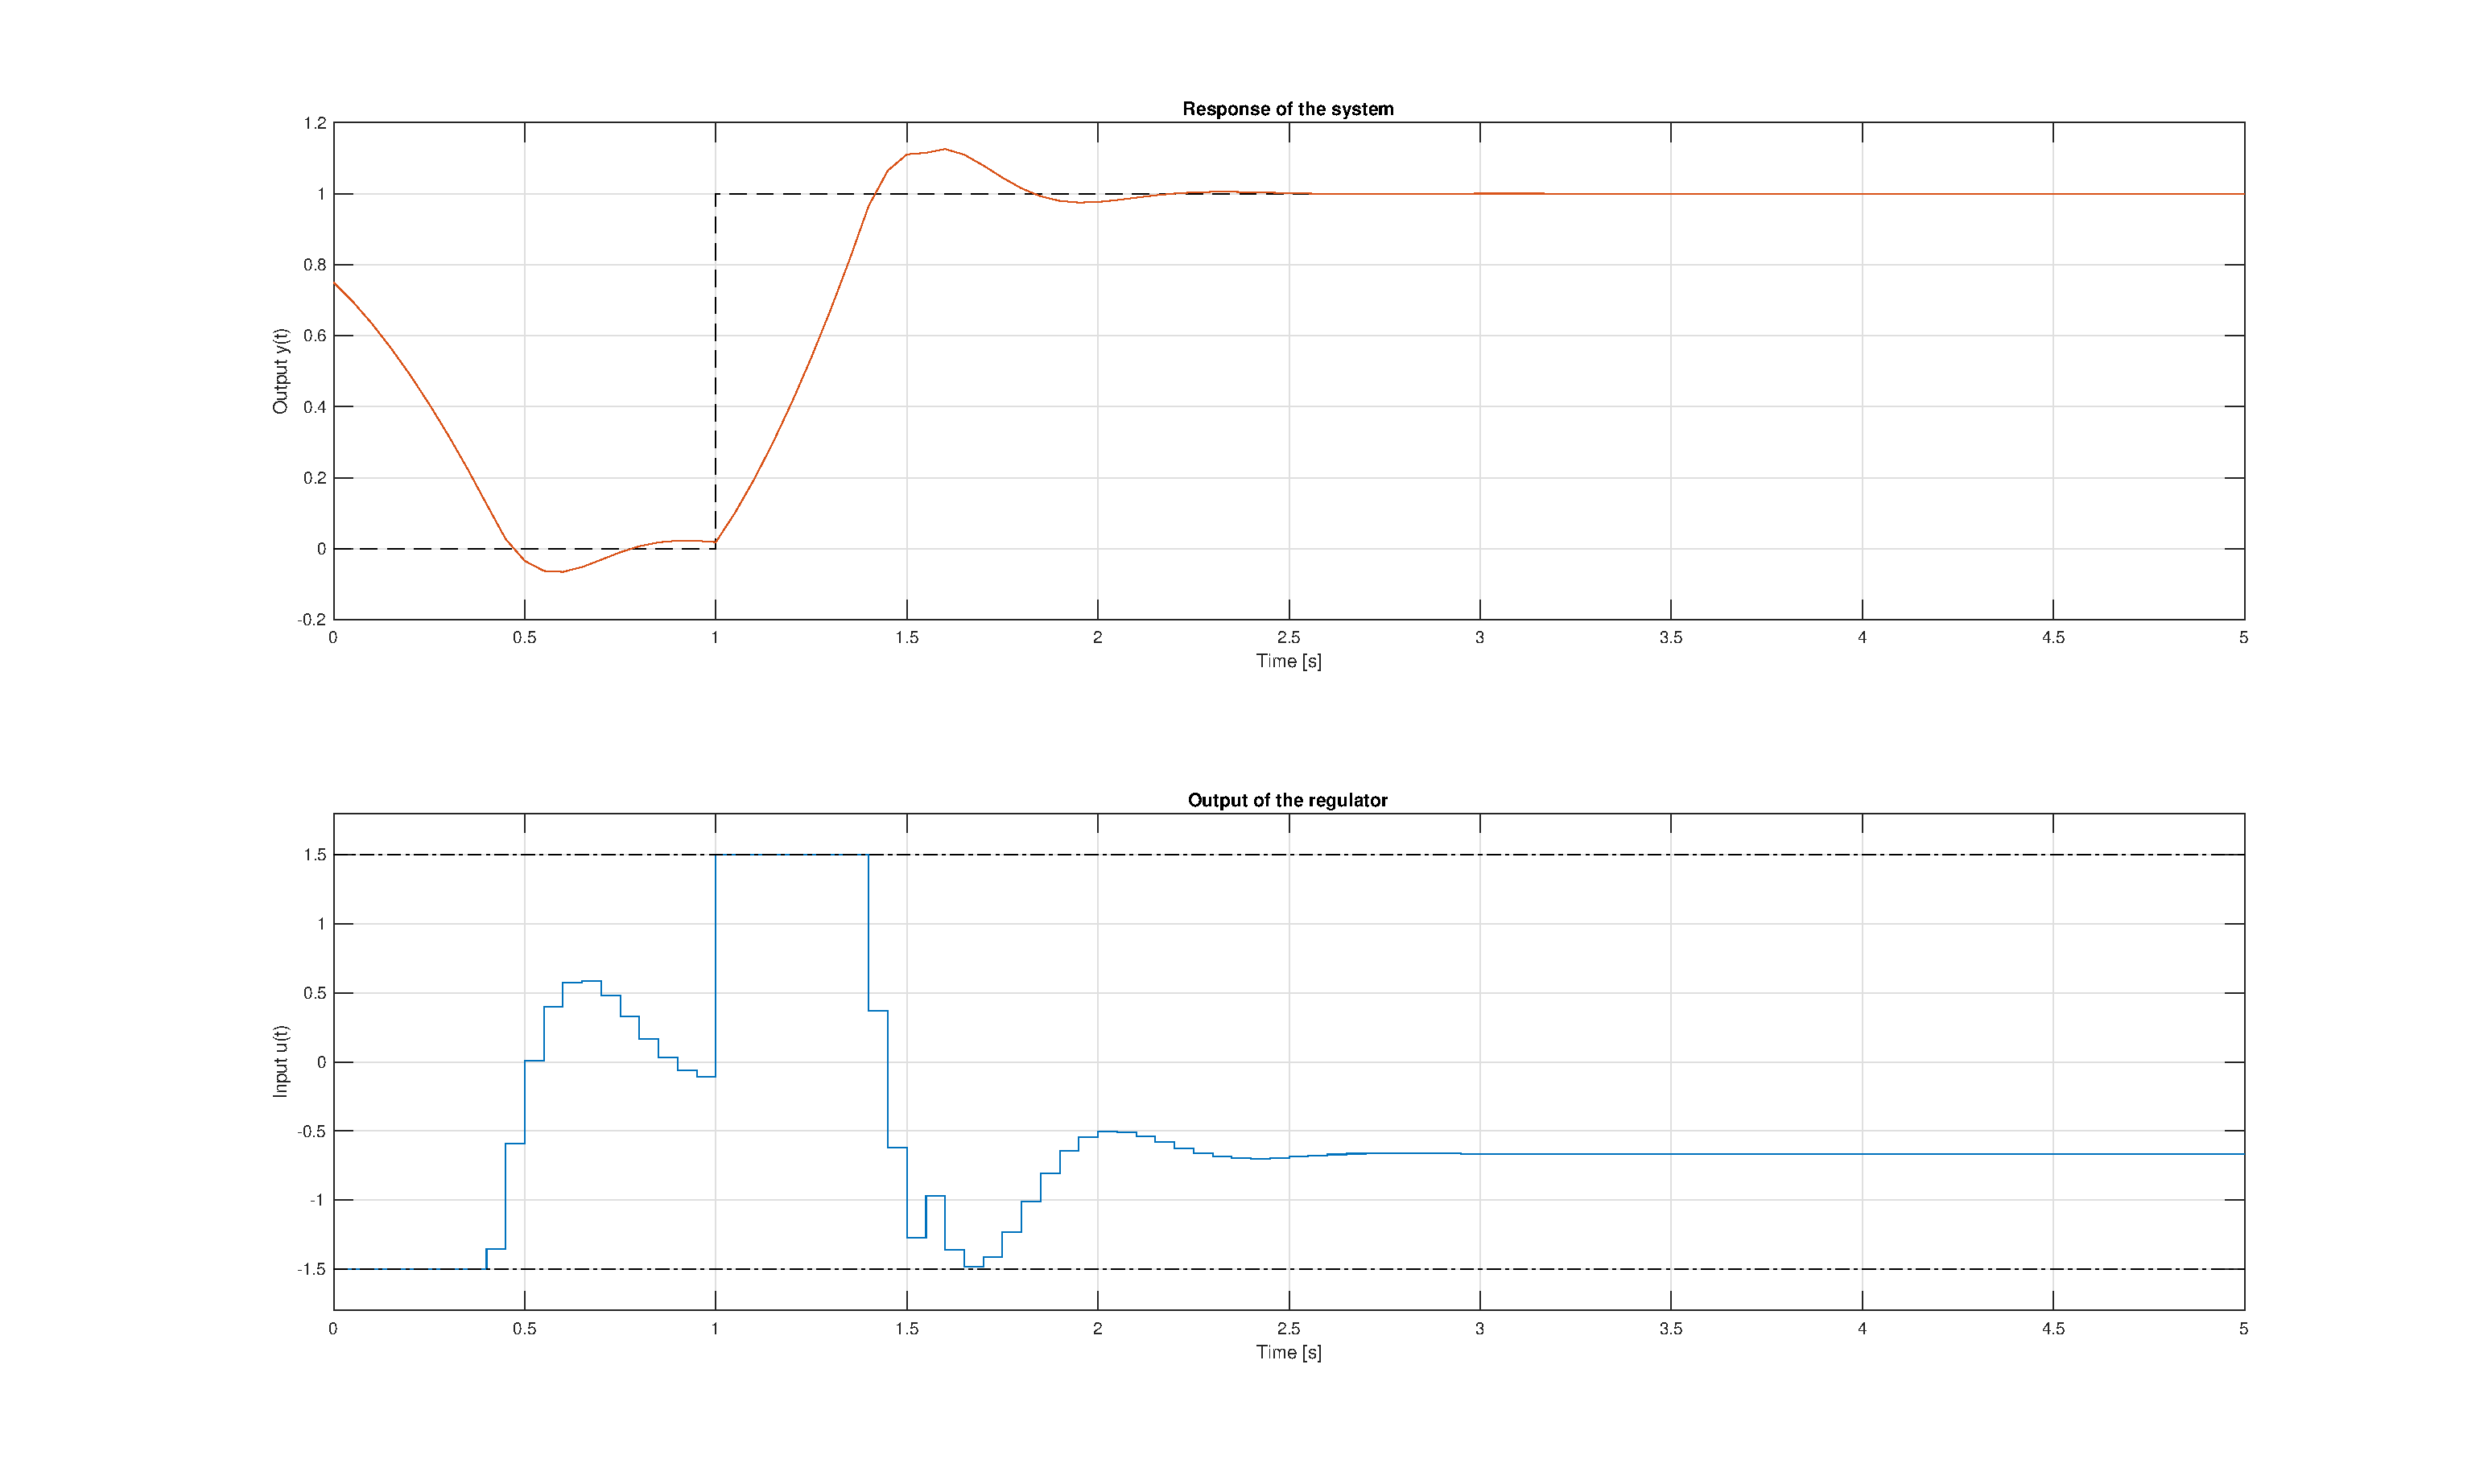
\includegraphics[clip, width=1.00\textwidth]{Response.eps}
        \caption{Odezva na jednotkový skor reference a výstup PI regulátoru}
        \label{fig:Model_1}
    \end{figure}
\end{itemize}



\end{document}
